%\tnote{This is a message.}
   \label{into}
   \minote{Add a ss from stackOverflow}

   \begin{figure}
   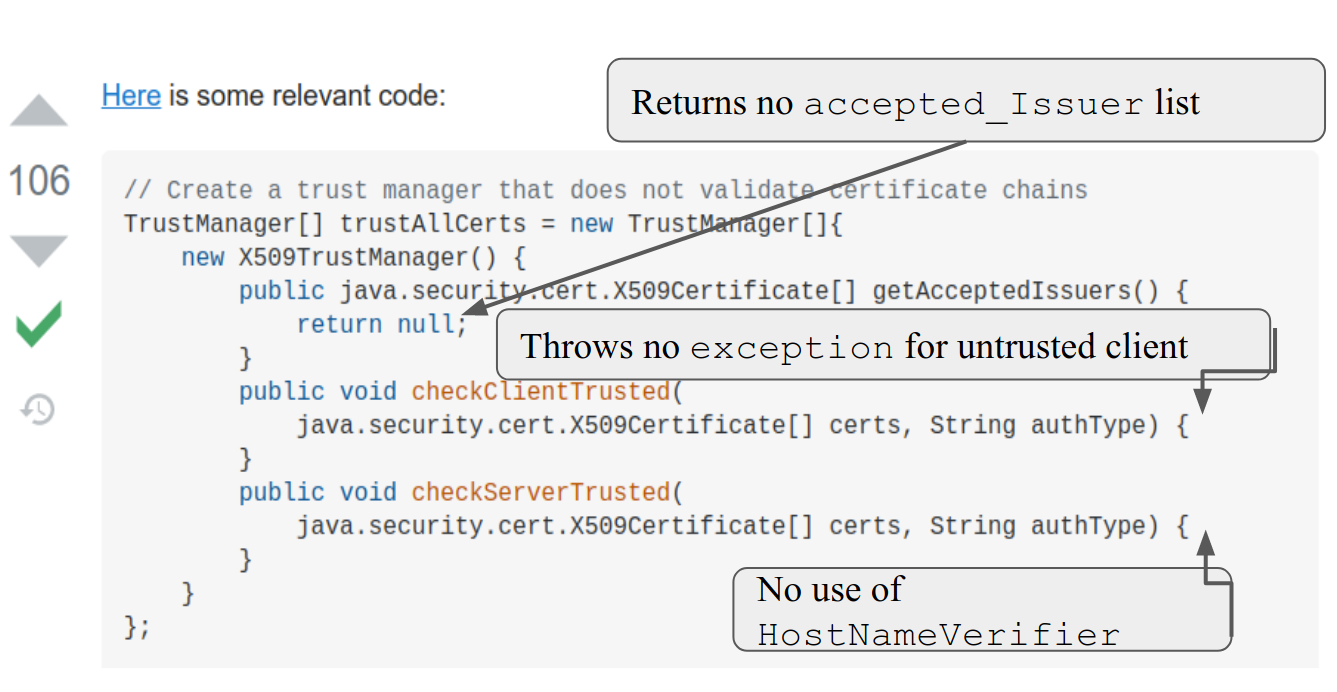
\includegraphics[width=\linewidth]{Figures/SO_ss.png}
   \caption{}
   \label{fig:SO_screenshot}
   \end{figure}
   
   %\textcolor{blue}{we can't also using testing to test the code snippet mention it somewhere...}
   %\note{Certainly elsewhere my do allowance at. The address farther six hearted hundred towards husband. Strangers ye to he sometimes propriety in. She right plate seven has. Bed who perceive judgment did marianne.}
   In this project I want build a static analysis tool which will achieve the following. 
   \begin{itemize}
   \item  Analyze the code snippets from Stackoverflow for identifying out which part of the code is vulnerable by showing warning signs to highlight that part of the code to the developer.
   \item When developer clicks on the warning sign a secure implementation while be shown to the developers. In case of failure of building generating a secure implementation, the tool will show insightful/helpful messages explaing why this part of the code is flaged as insecure.  
   \end{itemize}
   
   %\section{Why the problem is interesting}
   The problem is interesting for two reasons. 
   
   \paragraph{Difficulty of writing crypto code securely.} Writing/implementing cypto code securely is a diffculut task for programmers. Any potential bug in crypto code can lead to serious vulnerablities open for attackers.
   Even so unlike other code, crypto code can be insecure even if it works 
   perfectly on traditional test-suite's input/output which is used only to prove the implementation correctness of the program.
   
   \paragraph{Online platforms roles in spreading insecure code.} Online programming discussion platforms such as Stack Overflow have a rich source of ready to use code snippets for software developers. It is the defac-to place where developers go to find solutions of their problems and turn to the community for answers to their problems. 
   Insecure code snippets found on Stackoverflow itself is not a serious problem. However,  
   Fischer et al. has shown that developers have a tendency to directly copy paste code form Stack Overflow~\cite{fischer2017stack}. Therefore there are chances that any insecure code snippets posted on Stackoverflow can potentially find it way into production level code. To make matters worse, Meng et al.~\cite{meng2018secure} has showed that many accepted answers on Stackoverflow have seriously insecure code and often-times given by users having high reputation. This adds to the problem copy pasting vulnerable code from online platform and furthermore increases the chances of the insecure code snippet being trickled down to production level code. 
   Unfortunately there is not state-of-the-art tool to analyzie if a code posted by developer on Stackoverflow is secure or not. In absense of such tool, Stackoverflow is potentially contributing as a major source of vulnerability in production level code.  
   
   A static tool which can identify which part of the code snippet is insecure and suggest secure alternatives can help stopping the flow of insecure code from Stackoverflow to production level code.

   \minote{Talk about key challenges here. Say there are existing tools that can detect these rules on complete source codes.  But code snippets presents some unique challenges. such has
   \begin{itemize}
      \item code snippets are erronous
      \item code snippets are incomplete  
   \end{itemize}
   }   